\documentclass[]{article}

% Imported Packages
%------------------------------------------------------------------------------
\usepackage{amssymb}
\usepackage{amstext}
\usepackage{amsthm}
\usepackage{amsmath}
\usepackage{enumerate}
\usepackage{fancyhdr}
\usepackage[margin=1in]{geometry}
\usepackage{graphicx}
\usepackage{parskip}
\usepackage{xcolor}
\usepackage{float}

\newcommand{\emptyline}{\phantom{} & \phantom{} \\}
%\usepackage{extarrows}
%\usepackage{setspace}
%------------------------------------------------------------------------------

% Header and Footer
%------------------------------------------------------------------------------
\pagestyle{plain}  
\renewcommand\headrulewidth{0.4pt}                                      
\renewcommand\footrulewidth{0.4pt}                                    
%------------------------------------------------------------------------------

% Title Details
%------------------------------------------------------------------------------
\title{Deliverable \#2}
\author{SE 3A04: Software Design II -- Large System Design}
\date{March 13, 2023}                               
%------------------------------------------------------------------------------

% Document
%------------------------------------------------------------------------------
\begin{document}

\maketitle\begin{center}
\noindent{\bf Tutorial Number:} T03\\
{\bf Group Number:} G8 \\
{\bf Group Members:} 
\begin{itemize} \centering
	\item Adam Mak
	\item Eric Chen
	\item Justin Ho
	\item Ahmad Hamadi
	\item Kevin Ishak
	\item Jonathan Jiang
\end{itemize}\end{center}

\section*{IMPORTANT NOTES}
\begin{itemize}
	%	\item You do \underline{NOT} need to provide a text explanation of each diagram; the diagram should speak for itself
	\item Please document any non-standard notations that you may have used
	\begin{itemize}
		\item \emph{Rule of Thumb}: if you feel there is any doubt surrounding the meaning of your notations, document them
	\end{itemize}
	\item Some diagrams may be difficult to fit into one page
	\begin{itemize}
		\item Ensure that the text is readable when printed, or when viewed at 100\% on a regular laptop-sized screen.
		\item If you need to break a diagram onto multiple pages, please adopt a system of doing so and thoroughly explain how it can be reconnected from one page to the next; if you are unsure about this, please ask about it
	\end{itemize}
	\item Please submit the latest version of Deliverable 1 with Deliverable 2
	\begin{itemize}
		\item Indicate any changes you made.
	\end{itemize}
	\item If you do \underline{NOT} have a Division of Labour sheet, your deliverable will \underline{NOT} be marked
\end{itemize}

\newpage
\section{Introduction}
\label{sec:introduction}
% Begin Section

\subsection{Purpose}
\label{sub:purpose}
% Begin SubSection
The purpose of this document is to give an overview on the system and architectural design of the carpool app. The objective is to take requirements mentioned from the \textbf{SRS} and transform it into an architecture that describes the app's top-level structure and identifies its components, which acts as a preliminary blueprint for development. The intended audience for this document includes software developers and engineers, systems design architects, and other potential stakeholders who may benefit from an understanding of the system design. 
% End SubSection

\subsection{System Description}
\label{sub:system_description}
% Begin SubSection
The system is organized into a multiple sections, each fulfilling a requirement of the product. The user authentication section shows the systems used to ensure only registered users can use the app. The update account section takes care of any changes a user may need to make to their personal information. The arrival response section handles the display of the fare, peer-passenger rating system, and point allocation/redemption system. The dispatch ride sub-system handles the initialization of carpool events and requests of passengers to participate in pre-existing carpool events. The database system houses the different databases that are used. Finally, the default home view section takes care of the main general screen, connecting to all the other sections. The sections, and the relationships between them are illustrated in the analysis class diagram. Detailed information on any boundary class, entity class, and controller class can be found in the CRC cards section and system architecture sections of the document. 

The document also describes the subsystems that the product will use, and the data architecture styles that will be utilized for these subsections Information regarding this can be found in section 3.2.
% End SubSection

\subsection{Overview}
\label{sub:overview}
% Begin SubSection
In Section 2 the composition and interaction of domain concepts is outlined via a descriptive model, which will be represented visually in the form of a analysis class diagram. 

Section 3 provides a simplified overview of the overall architectural design and a simplified overview of all the subsystems that needs to be present in the final product. 

Section 4 goes further in-depth into the identified classes mentioned in Section 2 by representing them as CRC cards. 

At the end of the document, there is a record which represents the division of labour of all contributors to this deliverable.

% End SubSection

% End Section

\pagebreak
\section{Analysis Class Diagram}
\label{sec:analysis_class_diagram}
% Begin Section
\begin{figure}[h]
	\centering
	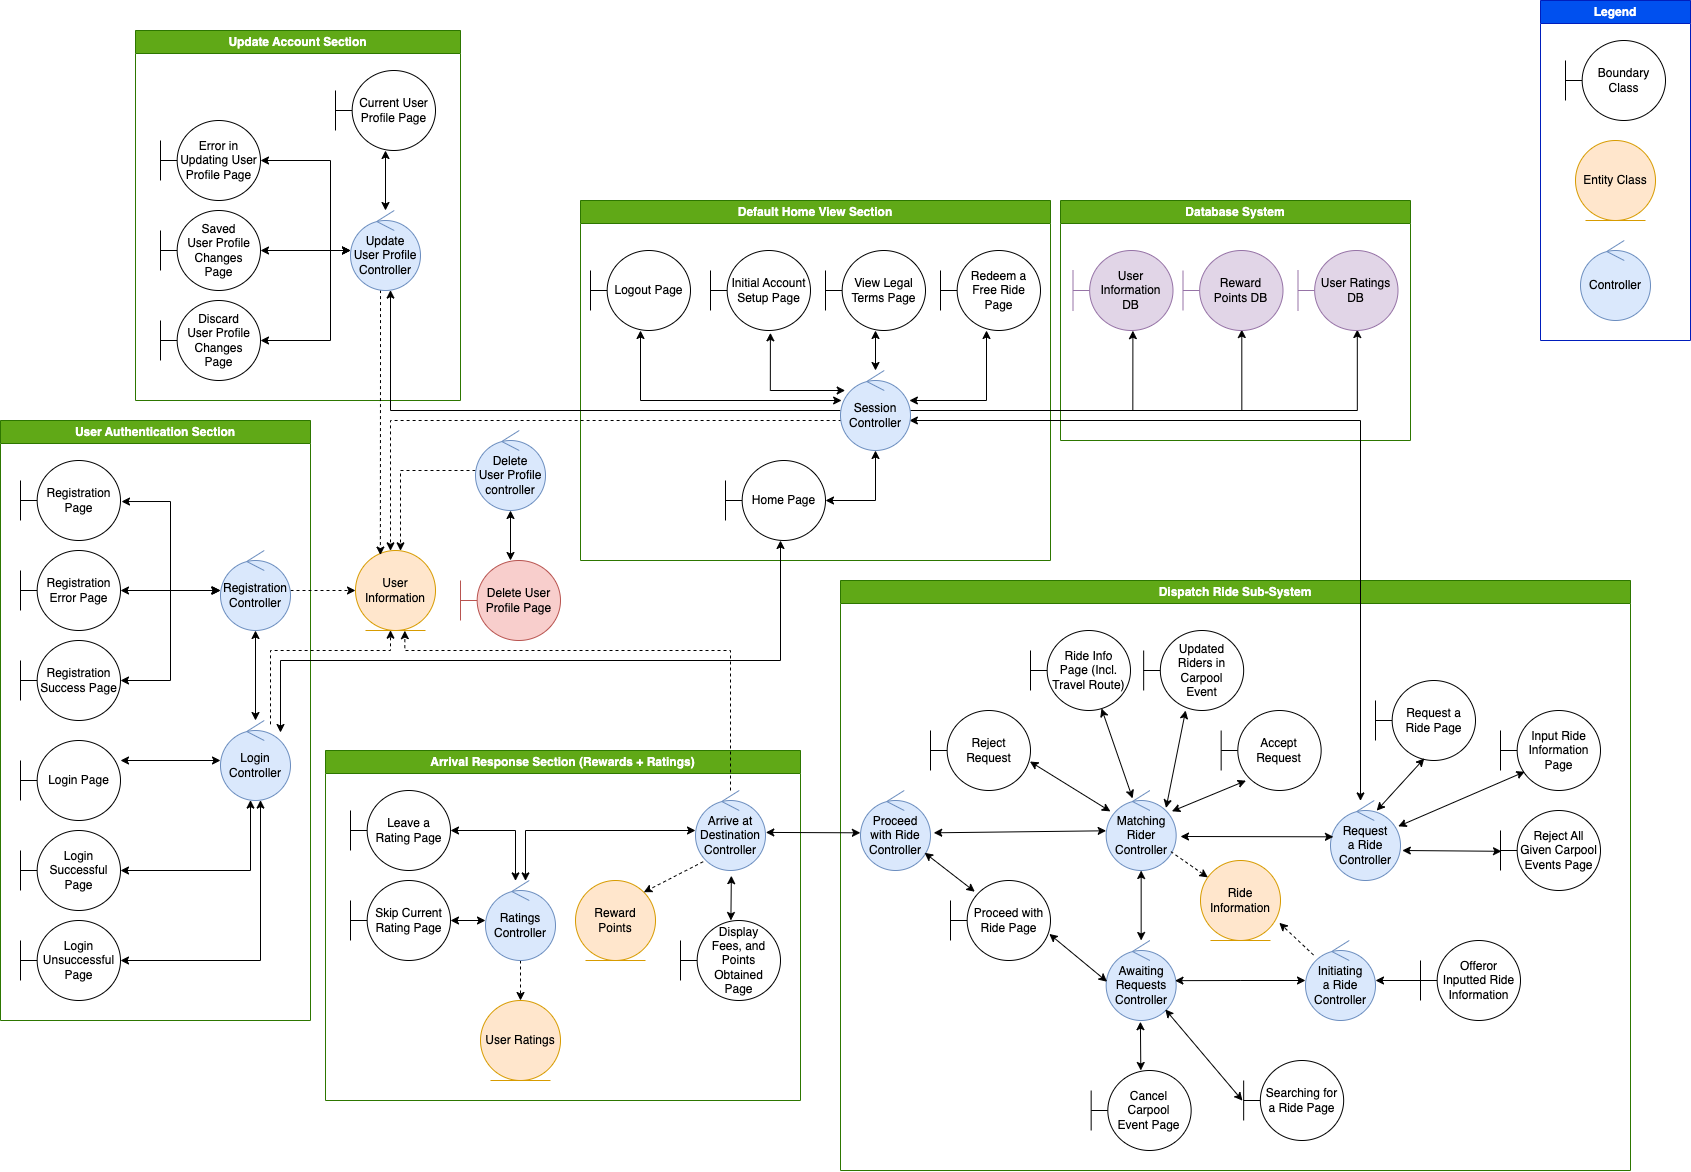
\includegraphics[width=49.5em]{D2/3a04_d2_analysis_class_diagram.drawio.png}
	\caption{Analysis Class Diagram (ACD) of the carpooling application.}
	\label{fig:acd}
\end{figure}
% End Section


\section{Architectural Design}
\label{sec:architectural_design}
% Begin Section

\subsection{System Architecture}
\label{sub:system_architecture}
% Begin SubSection
\begin{itemize}
	\item Identify and explain the overall architecture of your system
	\item Be sure to clearly state the name of the architecture you used (this is the name of the architectural pattern, not the name of your system)
	\item Provide the reasoning and justification of the choice of architecture
	\item Provide a structural architecture diagram showing the relationship among the subsystems (if appropriate)
	\item List any design alternatives you considered, but eliminated (and explain why you eliminated them)
\end{itemize}

The overall system will have a model view controller (MVC) architecture. Although the system involves storing and accessing data, how the data will be communicated will differ between subsystems (listed in Section 3.2). Here we are focusing more on the interaction between the user and internal workings of the application.

The MVC architecture separates the application into three components:
\begin{itemize}
    \item Model: The model represents the data and most of the business logic in the application. The model would contain the following components:
    \begin{itemize}
        \item User information: This includes information such as name, email, phone number, and password. This is encapsulated from the user.
        \item Ride information: This includes the details of users who are looking for or offering a ride, such as their starting location, destination, date, time, and number of available seats in the taxi.
        \item Reward points: These are associated with a user and are updated every time a user goes on a carpool ride.
        \item User ratings
    \end{itemize}
    \item View: Responsible for displaying the data to the user and receiving user input. It forwards input from the user to the controller and displays any input upon the controller's request to the user. These are a few components that will be included with the view:
    \begin{itemize}
        \item Login page: This allows users to log in to their accounts.
        \item Registration page: This allows users to create a new account.
        \item Home page: This shows the user's profile information and allows them to request or offer rides.
        \item Ride request page: This allows users to request a ride by specifying their starting location, destination, date, and time.
        \item Ride offer page: This allows users to offer a ride by specifying their starting location, destination, date, time, and number of available seats.
        \item Match page: This displays a list of potential matches between ride requests and offers (in the viewpoint of a requester).
    \end{itemize}
    \item Controller: Acts as a mediator between the model and the view. It handles user input, updates the model, and updates the view accordingly. It also deals with some business logic in tandem with the model. The controller would include some of the following components:
    \begin{itemize}
        \item Authentication controller: This handles user authentication, including login and sign-up.
        \item Profile controller: This handles the user's profile information.
        \item Ride request/offer controller: This handles the creation and retrieval of ride requests/offers.
        \item Dispatcher: This handles the matching of ride requests and offers and updates the view accordingly.
    \end{itemize}
    Note that some of these controllers are split up into sub-controllers in the analysis class diagram.
\end{itemize}

Having an system that separates components into sections that focus on different aspects of the application prioritizes separation of concerns. Each section has a specific responsibility and can be developed, tested, and maintained without having to worry too much about the other sections. 

An organized system also reduces complexity and improves understandability from a developer's perspective. This will in turn improve scalability and quicken the development process.

The presentation abstraction control (PAC) architecture was also considered as it is similar to the MVC architecture. In this context, each PAC agent would represent a subsystem in our application. We found that since the presentation and abstraction do not communicate with each other, it limits flexibility in the implementation and increases the workload and complexity of the control. Furthermore, since the controls in each agent communicate with each other, scaling the application may be tougher as it needs to consider all agents. Therefore, we eliminated the PAC architecture.


\begin{figure}[h]
	\centering
	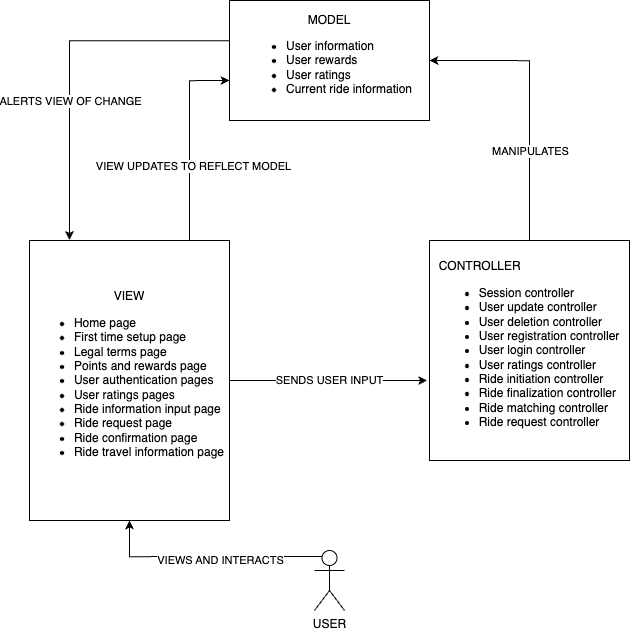
\includegraphics[width=30 em]{D2/3a04_d2_mvc.png}
	\caption{MVC Structural architecture diagram}
	\label{fig:acd}
\end{figure}
% End Section

% End SubSection

\subsection{Subsystems}
\label{sub:subsystems}
% Begin SubSection

There are 2 major subsystems that make up the overall system - the account system and the ride system.

\begin{itemize}
    \item User Account Management Subsystem \\
    \textbf{Purpose:} The purpose of this subsystem is to provide a separation of concerns between the business logic of the account management system and the database storage layer. User authentication, registration, modification, information, ratings, and rewards are handled by this subsystem. This also permits functionality such as encryption in the various data requests and modification made by the application required in the implementation of user accounts. This subsystem also makes it easier to test the application as the functional code can be tested in isolation of the database through abstraction using a repository layer. \\
    \textbf{Architecture:} This subsystem will have a repository architecture style. Account info from all users will be stored in a centralized data store in the form of a relational database. Data will only be stored or pulled upon request from the other components such as the account controller via a DBMS. In the implementation of the app, repositories will be created for user information, ratings, and rewards. Each repository would have methods which allow for the retrieval and modification of data which could then be used by the Ride subsystem in its functionality. 
\end{itemize}

\begin{itemize}
    \item Ride Subsystem \\
    \textbf{Purpose:} The primary purpose of this subsystem involves ride matchmaking, where carpoolers are matched with passengers based on location, route, and other potential criteria. The subsystem is also responsible for fare calculation, and is linked to the rating function. \\
    \textbf{Architecture:} This subsystem will make use of a blackboard architecture design. Regarding the blackboard components, the blackboard itself would contain the data required for the ride matchmaking functions, which would include carpooler and passenger information such as location. The knowledge sources of the blackboard would be the matchmaking methods and algorithms which utilize the data of the blackboard. The control mechanisms would be the methods which manage the interaction of the knowledge sources with the blackboard. An example of this would be methods that update the blackboard when certain events occur, such as removing carpoolers from the available rides list when their ride is initiated. 
\end{itemize}

% End SubSection

% End Section
	
\section{Class Responsibility Collaboration (CRC) Cards}
\label{sec:class_responsibility_collaboration_crc_cards}
% Begin Section
%registrationPage
\begin{table}[H]
        \centering
        \begin{tabular}{|p{5cm}|p{5cm}|}
        \hline 
         \multicolumn{2}{|l|}{\textbf{Class Name:} RegisterationPage} \\
        \hline
        \textbf{Responsibility:} & \textbf{Collaborators:} \\
        \hline
        Display the registration form &  \phantom{} \\
        \hline
        Allow user to select "register" or  "log in" & \phantom{} \\
        \hline
        Send request to register account to \textbf{RegistrationController} & \textbf{RegistrationController} \\
        \hline
        Know \textbf{RegistrationController} & \phantom{} \\
        \hline
        \end{tabular}
    \end{table}

%registrationErrorPage
\begin{table}[H]
    \centering
    \begin{tabular}{|p{5cm}|p{5cm}|}
        \hline 
         \multicolumn{2}{|l|}{\textbf{Class Name:} RegistrationErrorPage} \\
        \hline
        \textbf{Responsibility:} & \textbf{Collaborators:} \\
        \hline
        Display error message for failed registration &  \phantom{} \\
        \hline
        Provide options to retry registration & \phantom{} \\
        \hline
        Await with \textbf{RegistrationController} to handle registration errors & \textbf{RegistrationController} \\
        \hline
        Know \textbf{RegistrationController} & \phantom{} \\
        \hline
        \end{tabular}
    \end{table}

\begin{table}[H]
        \centering
        \begin{tabular}{|p{5cm}|p{5cm}|}
        \hline 
         \multicolumn{2}{|l|}{\textbf{Class Name:} RegisterationSuccessPage} \\
        \hline
        \textbf{Responsibility:} & \textbf{Collaborators:} \\
        \hline
        Display the Succesful registration form &  \phantom{} \\
        \hline
         Collect user input and pass it to the \textbf{RegistrationController} to store & \textbf{RegistrationController} \\ 
        \hline
        Know \textbf{RegistrationController} & \phantom{} \\
        \hline
        \end{tabular}
    \end{table}
    
\begin{table}[H]
        \centering
        \begin{tabular}{|p{5cm}|p{5cm}|}
        \hline 
         \multicolumn{2}{|l|}{\textbf{Class Name:} RegisterationController} \\
        \hline
        \textbf{Responsibility:} & \textbf{Collaborators:} \\
        \hline
       Receive user input for registration information (name, email, password, etc.). &  \textbf{RegistrationPage} \\
        \hline
       Validate the user input to ensure it meets certain requirements & \textbf{RegistrationSuccessPage} , \textbf{RegistrationErrorPage} \\ 
        \hline
        Create a new user account in the CustomerInfo database with the provided registration & \textbf{UserInformationDB} \\ 
        \hline
        Allow user account to be logged in with &\textbf{LoginController}\\
        \hline
        Know \textbf{UserInformationDB} & \phantom{} \\
        \hline
        Know \textbf{LoginController} & \phantom{} \\
        \hline
        \end{tabular}
    \end{table}

    %loginPage
   \begin{table}[H]
        \centering
        \begin{tabular}{|p{5cm}|p{5cm}|}
        \hline 
         \multicolumn{2}{|l|}{\textbf{Class Name:} LoginPage} \\
        \hline
        \textbf{Responsibility:} & \textbf{Collaborators:} \\
        \hline
        Display login form &  \phantom{} \\
        \hline
        Allow user to input login information and select "log in" & \phantom{} \\
        \hline
        Send request to validate credentials to \textbf{LoginController} & \textbf{LoginController} \\
        \hline
        Know \textbf{LoginController} & \phantom{} \\
        \hline
        \end{tabular}
    \end{table}

    \begin{table}[H]
        \centering
        \begin{tabular}{|p{5cm}|p{5cm}|}
        \hline 
         \multicolumn{2}{|l|}{\textbf{Class Name:} LoginUnSuccesfulPage} \\
        \hline
        \textbf{Responsibility:} & \textbf{Collaborators:} \\
        \hline
        Display to the user that login was unsuccessful &  \phantom{} \\
        \hline
        Send request to LoginController about the error that occurred during user  login &  \textbf{LoginController}
      \phantom{} \\
        \hline
        Know \textbf{LoginController} & \phantom{} \\
        \hline
        
        \end{tabular}
    \end{table}

    \begin{table}[H]
        \centering
        \begin{tabular}{|p{5cm}|p{5cm}|}
        \hline 
         \multicolumn{2}{|l|}{\textbf{Class Name:} LoginSuccesfulPage} \\
        \hline
        \textbf{Responsibility:} & \textbf{Collaborators:} \\
        \hline
        Display to the user that login was successful &  \phantom{} \\
        \hline
        Send request to LoginController to login &  \textbf{LoginController}
      \phantom{} \\
        \hline
        Know \textbf{LoginController} & \phantom{} \\
        \hline
        
        \end{tabular}
    \end{table}

     \begin{table}[H]
        \centering
        \begin{tabular}{|p{5cm}|p{5cm}|}
        \hline 
         \multicolumn{2}{|l|}{\textbf{Class Name:} LoginController} \\
        \hline
        \textbf{Responsibility:} & \textbf{Collaborators:} \\
        \hline
        Redirect user to home page after successful login & \textbf{HomePage},  \textbf{LoginSuccesfulPage}  \\
        \hline
       Redirect user to login unsuccessful page after unsuccessful login & \textbf{LoginUnsuccessfulPage} \\
        \hline
        Receive login request from \textbf{LoginPage} & \textbf{LoginPage}\\
        \hline
        Receive registration request from \textbf{LoginPage} & \textbf{RegistrationController} \\
        \hline
        Receive user info from \textbf{userInformationDB} & \textbf{UserInformation} \\
        \hline
        Know \textbf{HomePage} & \phantom{} \\
        \hline
        
        \end{tabular}
    \end{table}


     \begin{table}[H]
        \centering
        \begin{tabular}{|p{5cm}|p{5cm}|}
        \hline 
         \multicolumn{2}{|l|}{\textbf{Class Name:} UserInformationDB} \\
        \hline
        \textbf{Responsibility:} & \textbf{Collaborators:} \\
        \hline
        Store user information &  \phantom{} \\
        \hline
        Send user info to LoginController &  \textbf{LoginController}\\
        \hline
        Receive request to create new user & \textbf{RegisterationController}\\
        \hline
        Recieves Updated user information (such as password, email, etc.) &  \textbf{UpdateUserProfileController}\\
        \hline
         Delete user information &  \textbf{DeleteUserProfileController}\\
         \hline
         Send location info to arriveAtDestinationController & \textbf{ArriveAtDestinationController}\\
         \hline
         Send info throughout the session & \textbf{SessionController}\\
         \hline
         Know \textbf{SessionController} & \phantom{} \\
        \hline
         Know \textbf{LoginController} & \phantom{} \\
        \hline
         Know \textbf{ArriveAtDestinationController} & \phantom{} \\
        \hline
        \end{tabular}
    \end{table}

     \begin{table}[H]
        \centering
        \begin{tabular}{|p{5cm}|p{5cm}|}
        \hline 
         \multicolumn{2}{|l|}{\textbf{Class Name:} UpdateUserProfileController} \\
        \hline
        \textbf{Responsibility:} & \textbf{Collaborators:} \\
        \hline
        Retrieve current user profile information from \textbf{UserInformationDB} & \textbf{UserInformationDB} \\
        \hline
        Display current user profile information on \textbf{CurrentUserProfilePage} & \textbf{CurrentUserProfilePage} \\
        \hline
        Allow user to edit and submit updated user profile information & \phantom{} \\
        \hline
        Validate user profile information updates & \textbf{SavedUserProfileChangesPage} \\
        \hline
        Update \textbf{UserInformationDB} with user profile information updates & \textbf{UserInformationDB} \\
        \hline
        Redirect to \textbf{ErrorInUpdatingProfilePage} if update fails & \textbf{ErrorInUpdatingProfilePage} \\
        \hline
        Redirect to \textbf{DiscardUserProfileChangesPage} if user cancels update & \textbf{DiscardUserProfileChangesPage} \\
        \hline
        Collaborate with \textbf{SessionController} to check user authentication & \textbf{SessionController} \\
        \hline
        Know \textbf{UserInformationDB} & \phantom{} \\
        \hline
         Know \textbf{CurrentUserProfilePage} & \phantom{} \\
        \hline
        Know \textbf{SavedUserProfileChangesPage} & \phantom{} \\
        \hline 
        
        
        
        \end{tabular}
    \end{table}


\begin{table}[H]
        \centering
        \begin{tabular}{|p{5cm}|p{5cm}|}
        \hline 
         \multicolumn{2}{|l|}{\textbf{Class Name:} CurrentUserProfilePage} \\
        \hline
        \textbf{Responsibility:} & \textbf{Collaborators:} \\
        \hline
        Display user profile information &  \phantom{} \\
        \hline
        Allow user receive from \textbf{UpdateUserProfileController}  and view updated profile information & \textbf{UpdateUserProfileController} \\
        \hline
        
        \end{tabular}
    \end{table}

    \begin{table}[H]
        \centering
        \begin{tabular}{|p{5cm}|p{5cm}|}
        \hline 
         \multicolumn{2}{|l|}{\textbf{Class Name:} ErrorInUpdatingtUserProfilePage} \\
        \hline
        \textbf{Responsibility:} & \textbf{Collaborators:} \\
        \hline
        Display an error message when updating the user profile fails & \phantom{} \\
        \hline
        Send info to allow the user to \textbf{UpdateUserProfileController} to try updating the user profile again & \textbf{UpdateUserProfileController} \\
        \hline
         Know \textbf{UpdateUserProfileController} & \phantom{} \\
        \hline
      
        \end{tabular}
    \end{table}
    

\begin{table}[H]
        \centering
        \begin{tabular}{|p{5cm}|p{5cm}|}
        \hline 
         \multicolumn{2}{|l|}{\textbf{Class Name:} SavedUserProfilechangedPage} \\
        \hline
        \textbf{Responsibility:} & \textbf{Collaborators:} \\
        \hline
        Display a confirmation message when the user's profile changes have been saved & \phantom{} \\
        \hline
        Send info back to \textbf{UpdateUserProfileController}  & \textbf{UpdateUserProfileController} \\
        \hline
         Know \textbf{UpdateUserProfileController} & \phantom{} \\
        \hline
        
        \end{tabular}
    \end{table}



\begin{table}[H]
        \centering
        \begin{tabular}{|p{5cm}|p{5cm}|}
        \hline 
         \multicolumn{2}{|l|}{\textbf{Class Name:} DiscardUserProfilechangedPage} \\
        \hline
        \textbf{Responsibility:} & \textbf{Collaborators:} \\
        \hline
       Display a confirmation message when the user's profile changes have been discarded & \phantom{} \\
        \hline
        Send to \textbf{UpdateUserProfileController} that is was deleted & \textbf{UpdateUserProfileController} \\
        \hline
        Know \textbf{UpdateUserProfileController} & \phantom{} \\
        \hline
        
        \end{tabular}
    \end{table}

\begin{table}[H]
        \centering
        \begin{tabular}{|p{5cm}|p{5cm}|}
        \hline 
         \multicolumn{2}{|l|}{\textbf{Class Name:} DeleteUserProfileController} \\
        \hline
        \textbf{Responsibility:} & \textbf{Collaborators:} \\
        \hline
        Receive a request to delete a user's profile & \phantom{} \\
        \hline
        Confirm the user's intention to delete their profile & \textbf{DeleterUserProfilePage}\\
        \hline
        Delete the user's profile information from \textbf{UserInformationDB} & \textbf{UserInformationDB} \\
        \hline
         Know \textbf{UserInformationDB} & \phantom{} \\
        \hline
        
        \end{tabular}
    \end{table}

\begin{table}[H]
        \centering
        \begin{tabular}{|p{5cm}|p{5cm}|}
        \hline 
         \multicolumn{2}{|l|}{\textbf{Class Name:} DeleteUserProfilePage} \\
        \hline
        \textbf{Responsibility:} & \textbf{Collaborators:} \\
        \hline
       Display a confirmation message for deleting the user's profile & \phantom{} \\
        \hline
        Allow the user to confirm their intention to delete their profile & \phantom{} \\
        \hline
        Send a request to \textbf{DeleteUserProfileController} to delete the user's profile & \textbf{DeleteUserProfileController} \\
        \hline
        Display a success message after the user's profile has been deleted & \phantom{} \\
        \hline
        Know \textbf{DeleteUserProfileController} & \phantom{} \\
        \hline
        
        \end{tabular}
    \end{table}


   \begin{table}[H]
    \centering
    \begin{tabular}{|p{5cm}|p{5cm}|}
    \hline 
     \multicolumn{2}{|l|}{\textbf{Class Name:} SessionController} \\
    \hline
    \textbf{Responsibility:} & \textbf{Collaborators:} \\
    \hline
    Create session for user upon successful login & \textbf{LoginController, UserInformationDB} \\
    \hline
    Check session for user upon each request &  \phantom{} \\
    \hline
    Allow you to traverse between different UI &  \phantom{} \\
    \hline
    Redirect user to the `HomePage` after successful setup & \textbf{HomePage} \\
    \hline
    Allow user to log out of session & \textbf{LogoutPage} \\
    \hline
    Create initial session for new user upon account creation & \textbf{InitialAccountSetup} \\
    \hline
    Display legal terms for user to review and accept & \textbf{ViewLegalTermsPage} \\
    \hline
    Send/direct user to Allow updating profile & \textbf{UpdateUserProfileController} \\
    \hline
    Store and retrieve user ratings, information and rewardPoints & \textbf{UserRatingsDB}, \textbf{UserInformationsDB}, \textbf{RewardsPointsDB}\\
    \hline
    Receive to Initiate and track user participation in rides & \textbf{RequestARideController} \\
    \hline
    Receive info to redeem points page after succesful trip & \textbf{RedeemAFreeRidePage} \\
    \hline
    Know \textbf{DeleteUserProfileController} & \phantom{} \\
    \hline
    Know \textbf{UpdateUserProfileController} & \phantom{} \\
    \hline

    \end{tabular}
\end{table}

\begin{table}[H]
    \centering
    \begin{tabular}{|p{5cm}|p{5cm}|}
    \hline 
     \multicolumn{2}{|l|}{\textbf{Class Name:} ViewLegalTermsPage} \\
    \hline
    \textbf{Responsibility:} & \textbf{Collaborators:} \\
    \hline
    Display legal terms for the user to review and accept & \phantom{} \\
    \hline
    Send confirmation of acceptance to \textbf{SessionController} & \textbf{SessionController} \\
    \hline
    Know \textbf{SessionController} & \phantom{} \\
        \hline
    
    \end{tabular}
\end{table}

\begin{table}[H]
    \centering
    \begin{tabular}{|p{5cm}|p{5cm}|}
    \hline 
     \multicolumn{2}{|l|}{\textbf{Class Name:} UserRatingsDB} \\
    \hline
    \textbf{Responsibility:} & \textbf{Collaborators:} \\
    \hline
    Store and manage ratings given by users for drivers and riders & \phantom{} \\
    \hline
    retreive from ratings information &  \textbf{RatingsController} \\
    \hline
    send data to \textbf{SessionController}\\
    \hline
     Know \textbf{SessionController} & \phantom{} \\
        \hline
    
    \end{tabular}
\end{table}

\begin{table}[H]
    \centering
    \begin{tabular}{|p{5cm}|p{5cm}|}
    \hline 
     \multicolumn{2}{|l|}{\textbf{Class Name:} HomePage} \\
    \hline
    \textbf{Responsibility:} & \textbf{Collaborators:} \\
    \hline
    Display home page with relevant information and options for users &  \phantom{} \\
    \hline
    Allow user to view/send their profile information & \textbf{SessionController} \\
    \hline
    Allow user to search for rides & \phantom{} \\
    \hline
    Allow user to create and manage ride requests and reservations & \phantom{} \\
    \hline
    Allow user to access their ride history & \phantom{} \\
    \hline
    Send request to log in to `LoginController` & \textbf{LoginController} \\
    \hline
    Know \textbf{SessionController}  & \phantom{} \\
    \hline
    Know \textbf{LoginController}  & \phantom{}\\
    \hline
    
    \end{tabular}
\end{table}

\begin{table}[H]
    \centering
    \begin{tabular}{|p{5cm}|p{5cm}|}
    \hline 
     \multicolumn{2}{|l|}{\textbf{Class Name:} LogoutPage} \\
    \hline
    \textbf{Responsibility:} & \textbf{Collaborators:} \\
    \hline
    Display confirmation message to the user that they are logging out &  \phantom{} \\
    \hline
    Allow user to confirm or cancel the log out operation & \phantom{} \\
    \hline
    Send request to end user session to \textbf{SessionController} & \textbf{SessionController} \\
    \hline
    Know \textbf{SessionController}  & \phantom{} \\
    \hline
    
    \end{tabular}
\end{table}

\begin{table}[H]
    \centering
    \begin{tabular}{|p{5cm}|p{5cm}|}
    \hline 
     \multicolumn{2}{|l|}{\textbf{Class Name:} InitialAccountSetupPage} \\
    \hline
    \textbf{Responsibility:} & \textbf{Collaborators:} \\
    \hline
    Display the initial account setup form to the user &  \phantom{} \\
    \hline
    Allow user to input their personal and payment information & \phantom{} \\
    \hline
    Send request to create user account and store information  & \textbf{SessionController} \\
    \hline
    send user to the `HomePage` after successful setup & \textbf{HomePage} \\
    \hline
     Know \textbf{SessionController}  & \phantom{} \\
    \hline
     Know \textbf{HomePageController}  & \phantom{} \\
    \hline
    \end{tabular}
\end{table}

\begin{table}[H]
        \centering
        \begin{tabular}{|p{5cm}|p{5cm}|}
        \hline 
         \multicolumn{2}{|l|}{\textbf{Class Name:} RedeemFreeRidePage} \\
        \hline
        \textbf{Responsibility:} & \textbf{Collaborators:} \\
        \hline
        Display the redeem free ride page &  \phantom{} \\
        \hline
        Allow user to enter their unique code to redeem a free ride & \phantom{} \\
        \hline
        send current info to \textbf{SessionController} to check user authentication & \textbf{SessionController} \\
        \hline
         Know \textbf{SessionController}  & \phantom{} \\
        \hline
        \end{tabular}
    \end{table}

\begin{table}[H]
    \centering
    \begin{tabular}{|p{5cm}|p{5cm}|}
        \hline 
        \multicolumn{2}{|l|}{\textbf{Class Name:} RideInformationDB} \\
        \hline
        \textbf{Responsibilities:} & \textbf{Collaborators:} \\
        \hline
        Store, update, query information about rides & \phantom{} \\
        \hline
        Allow Retreival of Ride Information & 
        \textbf{InitiatingARideController} \\ 
        \hline
        Send information to \textbf{MatchingARideController} to match a ride using the data &  \textbf{MatchingARideController}\\
        \hline
        Know \textbf{MatchingARideController}  & \phantom{} \\
        \hline
        
    \end{tabular}
\end{table}

\begin{table}[H]
    \centering
    \begin{tabular}{|p{5cm}|p{5cm}|}
    \hline 
     \multicolumn{2}{|l|}{\textbf{Class Name:} RequestARideController} \\
    \hline
    \textbf{Responsibility:} & \textbf{Collaborators:} \\
    \hline
    Handle user requests to partake in a ride &  \phantom{} \\
    \hline
    Retrieve ride information from \textbf{InputRideInformationPage} & \textbf{InputRideInformationPage} \\
    \hline
    Retrieve user session information from \textbf{SessionController} & \textbf{SessionController} \\
    \hline
    Retrieve available rides from \textbf{RequestARidePage} & \textbf{RequestARidePage} \\
    \hline
    Notify user of successful ride request & \phantom{} \\
    \hline
    Notify user of unsuccessful ride request & \phantom{} \\
    \hline
    Allow user to select all carpool events for rejection & \textbf{RejectAllGivenCarpoolEventsPage}\\ 
    \hline
    send information to \textbf{MatchingRiderController} so it can match rides for current info provided &\textbf{MatchingRiderController}\\
    \hline
    Know \textbf{MatchingRiderController}  & \phantom{} \\
    \hline
    
    \end{tabular}
\end{table}

\begin{table}[H]
    \centering
    \begin{tabular}{|p{5cm}|p{5cm}|}
        \hline 
        \multicolumn{2}{|l|}{\textbf{Class Name:} InputRideDestinationPage} \\
        \hline
        \textbf{Responsibility:} & \textbf{Collaborators:} \\
        \hline
        Get destination input from user & \textbf{RequestInARideController} \\
        \hline
        Display map and route options to user & \Phantom{} \\
        \hline
        Display estimated ride cost to user & \Phantom{} \\
        \hline
        
    \end{tabular}
\end{table}


\begin{table}[H]
    \centering
    \begin{tabular}{|p{5cm}|p{5cm}|}
        \hline 
        \multicolumn{2}{|l|}{\textbf{Class Name:} RequestARidePage} \\
        \hline
        \textbf{Responsibility:} & \textbf{Collaborators:} \\
        \hline
        Display form for user to request a ride & \\
        \hline
        Send and Handle user request to place order & \textbf{RequestInARideController}  \\
        \hline
        Know \textbf{RequestInARideController}  & \phantom{} \\
    \hline
    \end{tabular}
\end{table}

\begin{table}[H]
    \centering
    \begin{tabular}{|p{5cm}|p{5cm}|}
        \hline 
        \multicolumn{2}{|l|}{\textbf{Class Name:} RejectAllGivenCarpoolEventsPage} \\
        \hline
        \textbf{Responsibility:} & \textbf{Collaborators:} \\
        \hline
        Display list of all carpool events for user to reject & \phantom{} \\
        \hline
        Allow user to select all carpool events for rejection & \phantom{} \\
        \hline
        Send request to \textbf{RequestARideController} to reject all selected carpool events & \textbf{RequestARideController} \\
        \hline
        Know \textbf{RequestInARideController}  & \phantom{} \\
    \hline
    \end{tabular}
\end{table}

\begin{table}[H]
    \centering
    \begin{tabular}{|p{5cm}|p{5cm}|}
    \hline 
     \multicolumn{2}{|l|}{\textbf{Class Name:} MatchingRideController} \\
    \hline
    \textbf{Responsibility:} & \textbf{Collaborators:} \\
    \hline
    Retrieve available ride information from \textbf{RideInformationDB} & \textbf{RideInformationDB} \\
    \hline
    Display available ride information on \textbf{RideInformationPage} & \textbf{RideInformationPage} \\
    \hline
    Accept a rider request to join a carpool event & \textbf{RideInformationDB}, \textbf{UpdatedRidersInCarpoolEvent} \\
    \hline
    Reject a rider request to join a carpool event & \textbf{RejectRequest} \\
    \hline
    Send info to Notify \textbf{AwaitingRequestsController} of accepted/rejected rider request & \textbf{AwaitingRequestsController} \\
    \hline
    Send info to collaborate with \textbf{ProceedWithRideController} to initiate a carpool event & \textbf{ProceedWithRideController} \\
    \hline
    Match riders with available drivers & \textbf{RequestInARideController} \\ 
    \hline
     Know \textbf{ProceedWithRideController}  & \phantom{} \\
    \hline
     Know \textbf{AwaitingRequestsController}  & \phantom{} \\
    \hline
    \end{tabular}
\end{table}

\begin{table}[H]
    \centering
    \begin{tabular}{|p{5cm}|p{5cm}|}
    \hline
    \multicolumn{2}{|l|}{\textbf{Class Name:} RejectRequest} \\
    \hline
    \textbf{Responsibility:} & \textbf{Collaborators:} \\
    \hline
    Allow user to reject &  \phantom{}\\
    Remove a ride request from the list of pending requests in \textbf{MatchingRideController} & \textbf{MatchingRideController} \\
    \hline
    Send and notify the user who submitted the rejected request & \textbf{MatchingRideController}
    \\
    \hline
     Know \textbf{MatchingRideController}  & \phantom{} \\
    \hline
    \end{tabular}
\end{table}

\begin{table}[H]
    \centering
    \begin{tabular}{|p{5cm}|p{5cm}|}
    \hline
    \multicolumn{2}{|l|}{\textbf{Class Name:} AcceptRequest} \\
    \hline
    \textbf{Responsibility:} & \textbf{Collaborators:} \\
    \hline
    Allow user to accept &  \phantom{}\\
    add a ride to  request from the list of pending requests in \textbf{MatchingRideController} & \phantom{} \\
    \hline
    Send info to Notify the user who submitted the accepted request to \textbf{MatchingRideController} & \textbf{MatchingRideController}
    \\
    \hline
     Know \textbf{MatchingRideController}  & \phantom{} \\
    \hline
    
    \hline
    \end{tabular}
\end{table}


\begin{table}[H]
    \centering
    \begin{tabular}{|p{5cm}|p{5cm}|}
    \hline
    \multicolumn{2}{|l|}{\textbf{Class Name:} RideInformationPage} \\
    \hline
    \textbf{Responsibility:} & \textbf{Collaborators:} \\
    \hline
    Display ride information to users and allow the to view available rides & \phantom{} \\
    \hline
    Send information about the ride so users can select and request a ride & \textbf{MatchingRideController} \\
    \hline
     Know \textbf{MatchingRideController}  & \phantom{} \\
    \hline
    
   
    \end{tabular}
\end{table}


\begin{table}[H]
    \centering
    \begin{tabular}{|p{5cm}|p{5cm}|}
        \hline 
        \multicolumn{2}{|l|}{\textbf{Class Name:} InitiatingARideController} \\
        \hline
        \textbf{Responsibility:} & \textbf{Collaborators:} \\
        \hline
        Create new ride offer with inputted information & \textbf{OfferorInputtedRideInformation} \\
        \hline
        Send Request to AwaitingRideController to wait forride requests & \textbf{AwaitingRideController} \\
        \hline
        Retreieve ride offer information in RideInformationDB  & \textbf{RideInformationDB } \\
        \hline
         Know \textbf{AwaitingRideController}  & \phantom{} \\
    \hline
    \end{tabular}
\end{table}

\begin{table}[H]
    \centering
    \begin{tabular}{|p{5cm}|p{5cm}|}
        \hline
        \multicolumn{2}{|l|}{\textbf{Class Name:} OfferorInputtedRideInformation} \\
        \hline
        \textbf{Responsibility:} & \textbf{Collaborators:} \\
        \hline
        Retrieve ride information inputted by offeror & \phantom{} \\
        \hline
        Send the info to \textbf{InitiatingARideController} to display success/error page upon successful submission & \textbf{InitiatingARideController} \\
        \hline
        Know \textbf{InitiatingRideController}  & \phantom{} \\
    \hline
        \end{tabular}
    \end{table}

\begin{table}[H]
    \centering
    \begin{tabular}{|p{5cm}|p{5cm}|}
        \hline 
        \multicolumn{2}{|l|}{\textbf{Class Name:} AwaitingRequestsController} \\
        \hline
        \textbf{Responsibility:} & \textbf{Collaborators:} \\
        \hline
        Send available ride requests to user on SearchingForARidePage & \textbf{SearchingForARidePage} \\
        \hline
        Initiate and track ride request in progress & \textbf{ProceedWithRidePage} \\
        \hline
        Receive Cancelled carpool event if no matches found & \textbf{CancelCarpoolEventPage} \\
        \hline
        Know \textbf{SearchingForARidePage}  & \phantom{} \\
    \hline
        
    \end{tabular}
\end{table}

\begin{table}[H]
    \centering
    \begin{tabular}{|p{5cm}|p{5cm}|}
        \hline 
        \multicolumn{2}{|l|}{\textbf{Class Name:} SearchingForARidePage} \\
        \hline
        \textbf{Responsibility:} & \textbf{Collaborators:} \\
        \hline
        Display search form for ride requests &  \phantom{} \\
        \hline
        Allow user to input search criteria and initiate search & \phantom{} \\
        \hline
        Await to display available ride requests to user & \textbf{AwaitingRequestsController} \\
        \hline
         Find a matching ride offer for user & \textbf{} \\
        \hline
    \end{tabular}
\end{table}


\begin{table}[H]
    \centering
    \begin{tabular}{|p{5cm}|p{5cm}|}
        \hline 
        \multicolumn{2}{|l|}{\textbf{Class Name:} ProceedWithRidePage} \\
        \hline
        \textbf{Responsibility:} & \textbf{Collaborators:} \\
        \hline
        Display ride details and options to proceed with ride &  \phantom{} \\
        \hline
        Allow user to select ride and initiate carpooling process & \textbf{ProceedWithRideController} \\
        \hline
         Send Process carpool request & \textbf{AwaitingRequestsController} \\
        \hline
         Know \textbf{AwaitingRequestController}  & \phantom{} \\
    \hline
    \end{tabular}
\end{table}

\begin{table}[H]
    \centering
    \begin{tabular}{|p{5cm}|p{5cm}|}
        \hline 
        \multicolumn{2}{|l|}{\textbf{Class Name:} CancelCarpoolEventPage} \\
        \hline
        \textbf{Responsibility:} & \textbf{Collaborators:} \\
        \hline
        Display ride details and options to cancel carpool event &  \phantom{} \\
        \hline
        Allow user to select carpool event to cancel & \phantom{} \\
        \hline
        Send Cancelled carpool event goes through the awaitingRequestsController & \textbf{AwaitingRequestsController} \\
        \hline
        Know \textbf{AwaitingRequestController}  & \phantom{} \\
    \hline
    \end{tabular}
\end{table}

\begin{table}[H]
    \centering
    \begin{tabular}{|p{5cm}|p{5cm}|}
    \hline
    \multicolumn{2}{|l|}{\textbf{Class Name:} ProceedWithRideController} \\
    \hline
    \textbf{Responsibility:} & \textbf{Collaborators:} \\
    \hline
    Send info Collaborate with \textbf{MatchingRideController} to match riders with drivers & \textbf{MatchingRideController} \\
    \hline
    Receive Display matched riders and ride information on \textbf{ProceedWithRidePage} & \textbf{ProceedWithRidePage} \\
    \hline
    Allow driver to start the ride and update ride status & \phantom{} \\
    \hline
    Receive Updated ride status and reward points & \textbf{ArriveAtDestinationController}\\
    \hline
     Know \textbf{MatchingRideController}  & \phantom{} \\
    \hline
    \end{tabular}
\end{table}

\begin{table}[H]
    \centering
    \begin{tabular}{|p{5cm}|p{5cm}|}
    \hline
    \multicolumn{2}{|l|}{\textbf{Class Name:} ArriveAtDestinationController} \\
    \hline
    \textbf{Responsibility:} & \textbf{Collaborators:} \\
    \hline
    Update user's rewards points in \textbf{RewardPointsDB} based on the ride information & \textbf{RewardPointsDB} \\
    \hline
    Display the fees charged for the ride and the points earned on \textbf{DisplayFeesAndPointsObtained} & \textbf{DisplayFeesAndPointsObtained} \\
    \hline
    Send request for user to leave a rating for the ride on \textbf{RatingController} & \textbf{RatingController} \\
    \hline
     Send info with \textbf{ProceedWithRideController} to finalize the ride & \textbf{ProceedWithRideController} \\
    \hline
    Know \textbf{ProceedWithRideController}  & \phantom{} \\
    \hline
    Know \textbf{RewardPointsDB}  & \phantom{} \\
    \hline
    Know \textbf{RatingController}  & \phantom{} \\
    \hline
    \end{tabular}
\end{table}

\begin{table}[H]
    \centering
    \begin{tabular}{|p{5cm}|p{5cm}|}
    \hline
    \multicolumn{2}{|l|}{\textbf{Class Name:} RewardPointsDB} \\
    \hline
    \textbf{Responsibility:} & \textbf{Collaborators:} \\
    \hline
    Store user's rewards points information & \phantom{} \\
    \hline
    Receive Updated user's rewards points information based on the ride information & \textbf{ArriveAtDestinationController} \\
    \hline
    Retrieve user's rewards points information for display & \phantom{} \\
    \hline
    \end{tabular}
\end{table}

\begin{table}[H]
    \centering
    \begin{tabular}{|p{5cm}|p{5cm}|}
    \hline
    \multicolumn{2}{|l|}{\textbf{Class Name:} DisplayFeesAndPointsObtainedPage} \\
    \hline
    \textbf{Responsibility:} & \textbf{Collaborators:} \\
    \hline
    Display the fees charged for the ride and the points earned & \textbf{ArriveAtDestinationController} \\
    \hline
    send Update display with the latest fees and points earned to \textbf{ArriveAtDestinationController} & \phantom{} \\
    \hline
     Know \textbf{ArriveAtDestinationController}  & \phantom{} \\
    \hline
    
    
    \end{tabular}
\end{table}


\begin{table}[H]
    \centering
    \begin{tabular}{|p{5cm}|p{5cm}|}
    \hline
    \multicolumn{2}{|l|}{\textbf{Class Name:} RatingsController} \\
    \hline
    \textbf{Responsibility:} & \textbf{Collaborators:} \\
    \hline
    Receive ride rating from user on \textbf{LeaveARatingPage} & \textbf{LeaveARatingPage} \\
    \hline
    Send and save the user's rating to \textbf{UserRatingsDB} & \textbf{UserRatingsDB} \\
    \hline
    Receive info and collaborate with \textbf{ArriveAtDestinationController} to be able to start the rating process & \textbf{ArriveAtDestinationController} \\ 
    \hline
    send user reuqest to skip rating for current ride on \textbf{SkipCurrentRatingPage} & \textbf{SkipCurrentRatingPage} \\
    \hline
    Know \textbf{SkipCurrentRatingPage}  & \phantom{} \\
    \hline
    Know \textbf{RewardPointsDB}  & \phantom{} \\
    \hline
    \end{tabular}
\end{table}

\begin{table}[H]
    \centering
    \begin{tabular}{|p{5cm}|p{5cm}|}
    \hline
    \multicolumn{2}{|l|}{\textbf{Class Name:} LeaveARatingPage} \\
    \hline
    \textbf{Responsibility:} & \textbf{Collaborators:} \\
    \hline
    Display rating form & \phantom{} \\
    \hline
    Allow user to input rating and select "submit" & \phantom{} \\
    \hline
    Send rating to \textbf{RatingsController} & \textbf{RatingsController} \\
    \hline
    Know \textbf{RatingsController}  & \phantom{} \\
    \hline
    \end{tabular}
\end{table}

\begin{table}[H]
    \centering
    \begin{tabular}{|p{5cm}|p{5cm}|}
    \hline
    \multicolumn{2}{|l|}{\textbf{Class Name:} SkipCurrentRatingPage} \\
    \hline
    \textbf{Responsibility:} & \textbf{Collaborators:} \\
    \hline
    Display a page allowing user to skip current ride rating & \phantom{} \\
    \hline
    Allow user to select "skip" to skip the current rating & \phantom{} \\
    \hline
    Send request to \textbf{RatingsController} to skip current rating & \textbf{RatingsController} \\
    \hline
     Know \textbf{RatingsController}  & \phantom{} \\
    \hline
    \end{tabular}
\end{table}



    

\appendix
\section{Division of Labour}
\label{sec:division_of_labour}
% Begin Section
\begin{center} \begin{tabular} {|c|p{35em}|}
	\hline
	\textbf{Team Member} & \textbf{Contribution} \\
	\hline \hline
	Adam Mak & Purpose, Overview, Architecture design (3.1) and subsystem architectures (3.2), resolving NFR feedback for D1 (added SR-P3)\\
	& Signed by: Adam Mak\\
	\hline
	Eric Chen & Analysis Class Diagram (ACD), Resolving BE feedback for D1 and updating changes to LaTeX document.\\
	& Signed by: Eric Chen\\
	\hline
	Justin Ho & Analysis Class Diagram (ACD), Resolving BE feedback for D1, updating changes to LaTeX document, section 1.2 (system description)\\
	& Signed by: Justin Ho\\
	\hline
	Ahmad Hamadi & CRC Cards, purpose(1.1), Overview(1.2), resolving feedback\\
	& Signed by: Ahmad Hamadi \\
	\hline
	Kevin Ishak & CRC Cards \\
	& Signed by: Kevin Ishak \\
	\hline
	Jonathan Jiang & Purpose, Structural architectural diagram, Subsystems\\
	& Signed by: Jonathan Jiang\\
	\hline
\end{tabular} \end{center}
% End Section


\end{document}
%------------------------------------------------------------------------------